\chapter{Introduction}

\section{Background}
Climbing as a human activity has been around for many hundreds of years, with the first development in specialized tools seen in the 15th century. Rock and mountain climbing were primarily necessity-driven until the mid-19th century when technological advancements allowed climbing to evolve into a more standardized sport. Accidents decreased with improved gear and standardized equipment. \\\\
In the last decade, rock climbing has seen a surge in participants, leading to increased demand for climbing gear from companies like Black Diamond and Mammut. With climbing’s inclusion in the 2020 and 2024 Summer Olympics, there is a growing need for innovative training methodologies and equipment advancements to support athletes in achieving peak performance \citep{Consuegra-2023}.

\begin{figure}[ht]
    \centering
    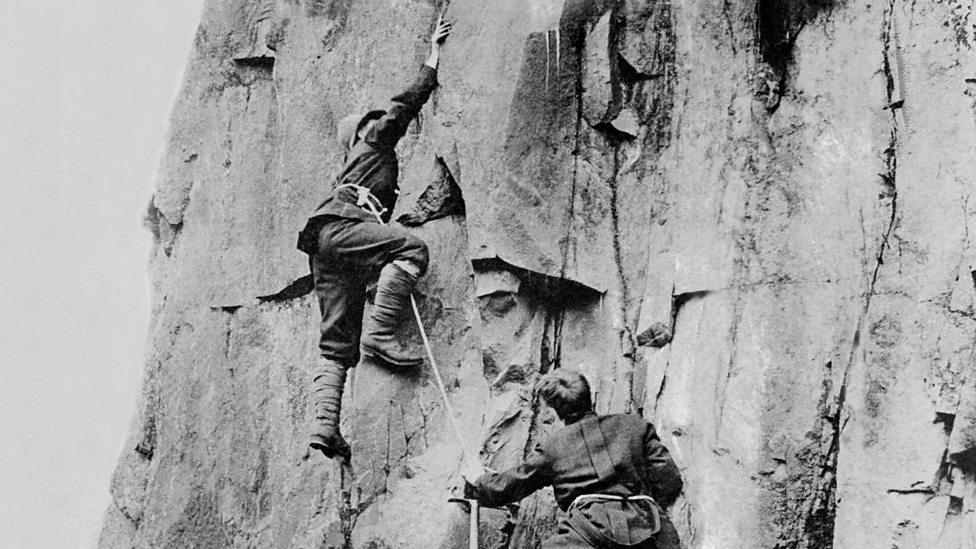
\includegraphics[width=0.75\linewidth]{figs/early-climbing.jpg}
    \caption{Early days of rock climbing}
\end{figure}

\section{Objectives}
The primary goal of this project is to conceptualize, design, and prototype a rotary climbing wall that revolutionizes endurance training for rock climbers. By providing a continuous rotating surface, this design simulates varying difficulties and overhang conditions, enhancing the indoor training experience for climbers.

\section{Motivation}
Indoor climbing facilities, particularly in South Africa, face spatial limitations that restrict the ability to train for endurance. Few climbing gyms offer high walls, limiting training opportunities for long-duration climbs. The development of a rotary climbing wall addresses this by providing an endless climbing surface, similar to a treadmill, enabling climbers to train on extended routes without the need for extensive vertical space.

\section{Problem Definition}
The primary challenge in rock climbing endurance training is the limitation of vertical space in indoor climbing gyms, particularly in regions like South Africa where facilities with high walls are scarce. Climbing endurance is a key component of performance, and current bouldering facilities, with walls of 4-5 meters, are insufficient for long-duration endurance training. \\\\
This project aims to solve this problem by developing a rotary climbing wall that offers a continuous climbing surface and simulates different difficulty levels and overhang conditions. The wall's rotating mechanism addresses the vertical space issue and provides climbers with the ability to train for endurance within a constrained space.

\section{Design Methodology}
The design methodology follows a systematic \textit{design, build, and test} approach, with the aim of addressing the problem outlined above. The methodology is divided into two main phases: conceptual design and detailed design.

\subsection{Phase I: Conceptual Design}
\begin{itemize}
    \item \textbf{Identification of Customer Needs:} Based on the problem definition, customer needs were identified to ensure the design aligns with the functional requirements of climbers who seek endurance training solutions.
    \item \textbf{Problem Definition:} The problem, as discussed in the previous section, focuses on the need for a continuous climbing surface to overcome vertical space limitations in traditional indoor climbing gyms.
    \item \textbf{Gathering Information:} A thorough review of technical articles, patents, and market solutions was conducted to inform the design. This is presented in Chapter \ref{chap:technology_review}.
    \item \textbf{Concept Generation:} Several design concepts were generated using creative brainstorming techniques. These concepts are detailed in Chapter \ref{chap:concept_design}.
    \item \textbf{Evaluation of Concepts:} The generated concepts were evaluated based on feasibility, cost, performance, and scalability.
    \item \textbf{Concept Integration:} The most suitable concept was selected and further refined into a comprehensive system design that addresses both functional and performance requirements.
    \item \textbf{Design Review:} A formal review of the final concept was conducted to ensure all requirements were met before transitioning to the detailed design phase.
\end{itemize}

\subsection{Phase II: Detailed Design}
\begin{itemize}
    \item \textbf{Design Verification:} The design was verified using structural and performance analysis, including Finite Element Method (FEM) simulations, to ensure it met safety and performance standards.
    \item \textbf{Detailed Engineering Drawings:} Engineering drawings were created to specify the dimensions, tolerances, and materials needed for manufacturing the rotary climbing wall.
\end{itemize}

\section{Use of Artificial Intelligence}
This report was composed in LaTeX, with AI assistance limited to spelling and grammar checks and enhancing the flow of certain paragraphs. Additionally, AI was used to support figure and table formatting in LaTeX but was not involved in the design, construction, or testing of the rotating climbing wall.

